\chapter{EMTG Options}
\label{chap:options}
An \ac{EMTG} mission is created through a text file known as an \ac{EMTG} Options file with the extension \verb|.emtgopt|. \ac{EMTG} Options files define the mission parameters as well as link to the ephemeris and hardware configuration needed for the mission. The ephemeris configuration is another text file known as an \ac{EMTG} Universe file with extension \verb|.emtg_universe|. Hardware configurations are stored in another set of text files for the launch vehicle and spacecraft with extensions \verb|.emtg_launchvehicleopt| and \verb|.emtg_spacecraftopt|. \ac{EMTG} Options files can be configured using a text editor or the PyEMTG \ac{GUI}. This chapter will discuss the \ac{EMTG} Options file and PyEMTG interface.

\noindent Most interaction with the \ac{EMTG} Options file can be accomplished through PyEMTG though some options are only present in the \verb|.emtgopt| file and must be changed there using a text editor. An \ac{EMTG} Options file can be created in PyEMTG by selecting "File, New, Mission" (Ctrl + m). An existing \ac{EMTG} Options file can be opened by selecting "File, Open" (Ctrl + o) and choosing an existing \verb|.emtgopt| file.

\begin{figure}[H]
    \centering
    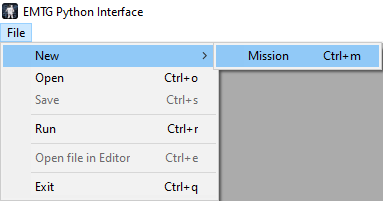
\includegraphics[width=0.5\textwidth]{../../shared_latex_inputs/images/pyemtg_file_new.png}
    \caption{Creating a new EMTG Options file}
\end{figure}

\noindent An \ac{EMTG} Options file is broken up into several sections shown with tabs in PyEMTG: Global Mission Options, Spacecraft Options, Journey Options, Solver Options, Physics Options, and Output Options. The rest of the chapter will cover each of the sections in turn as well as the options that can only be accessed through the \verb|.emtgopt| text file.

\begin{figure}[H]
    \centering
    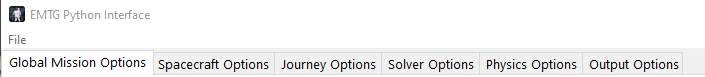
\includegraphics[width=0.9\textwidth]{../../shared_latex_inputs/images/pyemtg_options_tabs.png}
    \caption{EMTG Options tabs}
\end{figure}